% !TEX root = ./rep.tex
\section{Demonstration simulation}
\label{s:demo}

We demonstrate here the use of cardinal on two pebble bed setups representative of FHR cores.

\subsection{146 Pebbles}
\label{ss:c4}

Using the Nek5000 model of the TAMU experiment as a basis, we have developed a multiphysics simulation of a bed comprising 146 pebbles.
The pebble model for Nek5000 reflects the practices used for the TAMU experiment, which were validated carefully against experimental PIV data. Inlet/outlet boundary conditions are used (Figure~\ref{f:pb2}). Unlike the TAMU experiment, here the mesh is designed to allow a clearance between pebbles. This facilitates the coupling but it will likely be updated in future simulations. The difference is outlined in Figure~\ref{f:pb2}. The mesh comprises approximately roughly 500,000 elements overall and it is designed to run at $N=5$ for coarse results and $N=7$ for finer simulations (for a max of 256 million grid points). We assume constant properties.

\begin{figure}[!h]
\centering
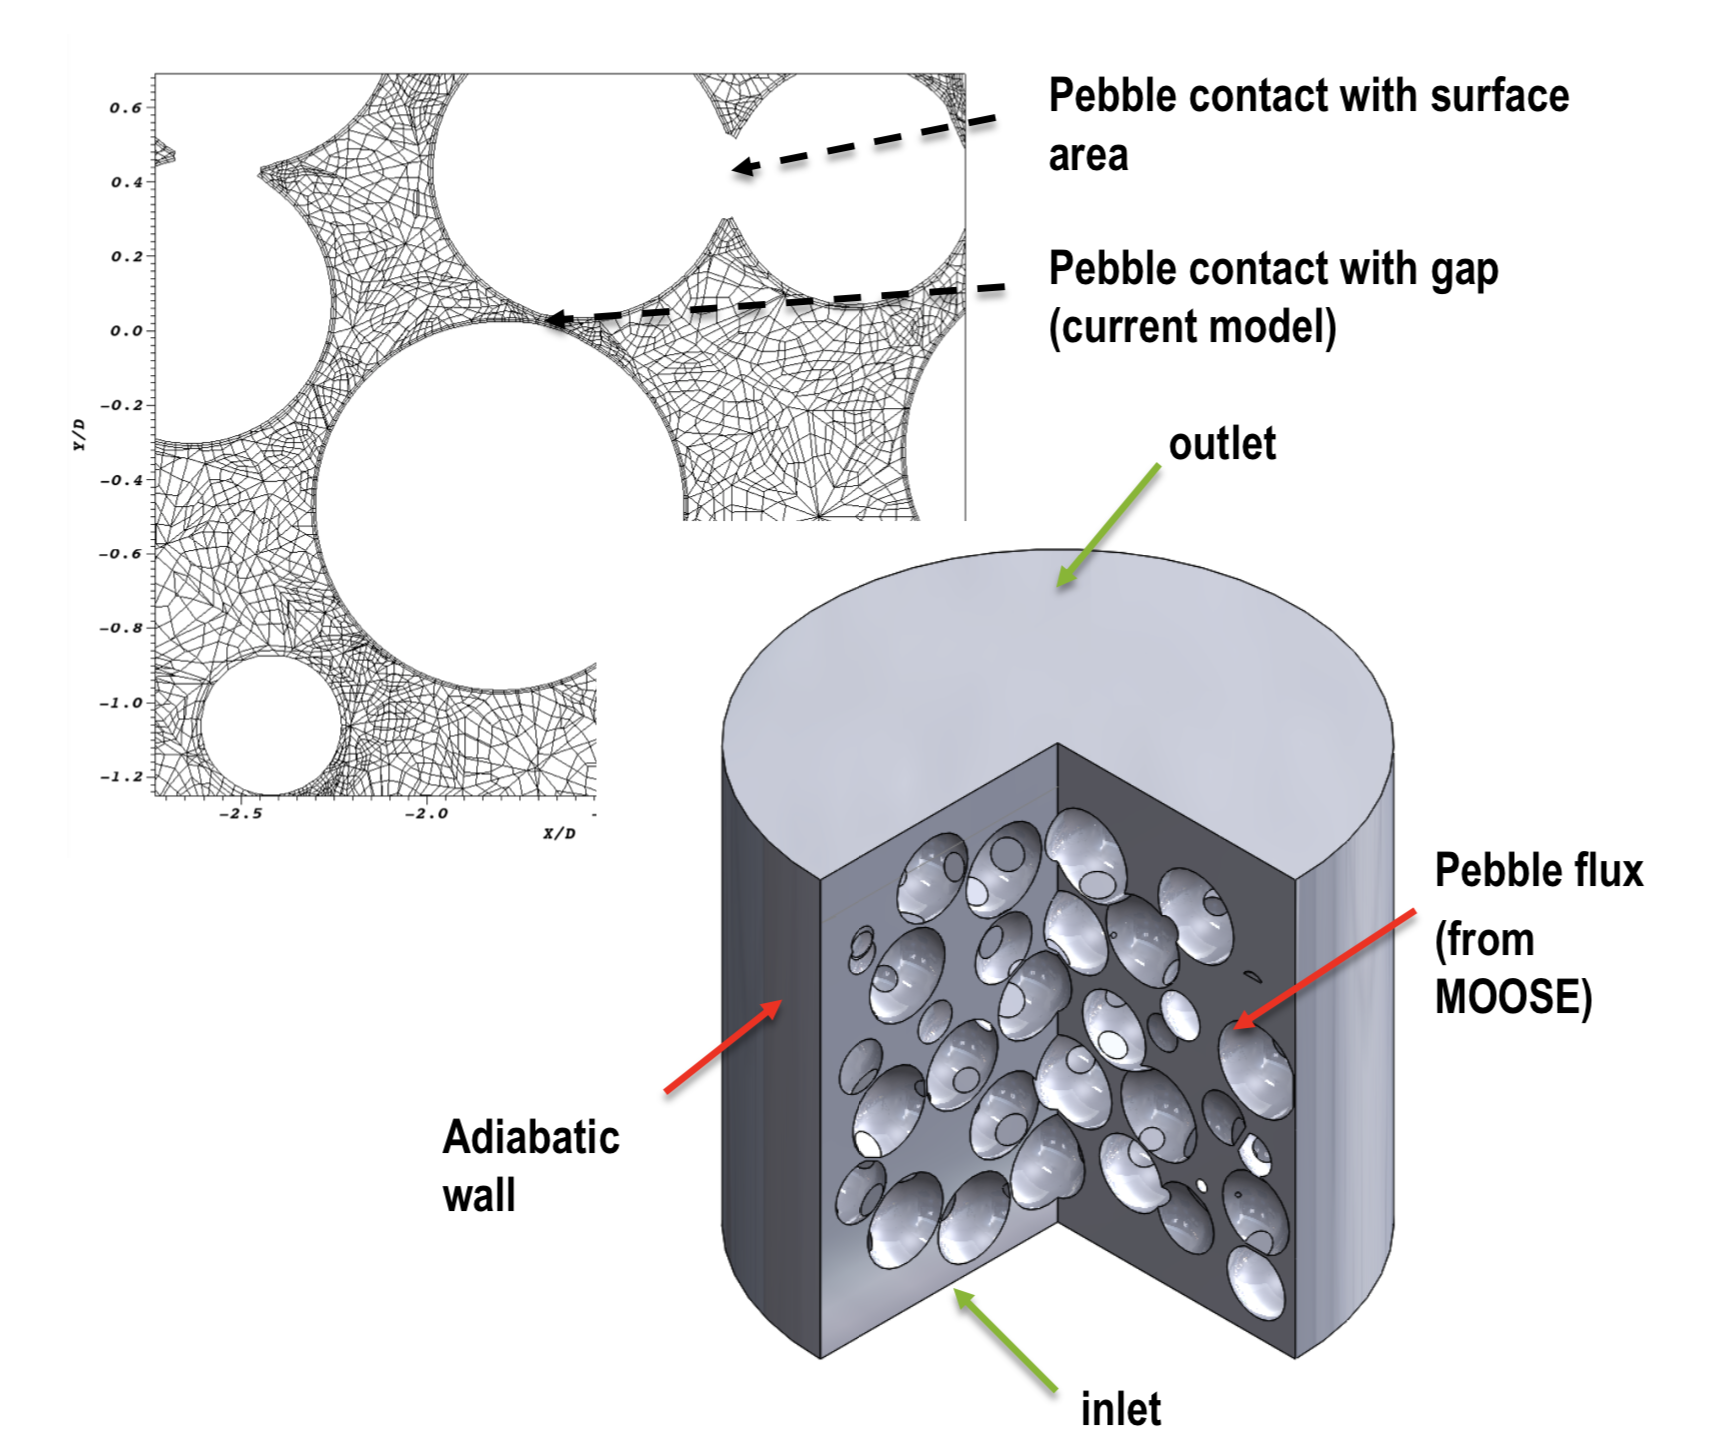
\includegraphics[clip=true,width=0.8\textwidth]{Figures/pb_mesh}
\caption{Mesh and boundary conditions for Nek5000 problem.}
\label{f:pb2}
\end{figure}

To test various options and accelerate the development we defined four variants of the demo problem all available in the Cardinal repository. The variants reflect the need to define cheaper transients for testing purposes. Table~\ref{tab:nek} shows the cases: they are listed in order of increasing computational cost. Restarting from an advanced restart leads to faster convergence. Moreover, simulating the full Navier-Stokes is considerably more expensive than assuming a ``frozen velocity'' and solving only the advection-diffusion equation.

\begin{table}
  \centering
  \begin{tabular}{|lcc|}
    \hline \hline
    Case & Restart condition & Solver \\
    \hline
    1 & Advanced restart state & Advection-Diffusion only \\
    2 & Constant temperature   & Advection-Diffusion only \\
    3 & Advanced restart state & Full Navier-Stokes \\
    4 & Constant temperature   & Full Navier-Stokes \\
    \hline \hline
  \end{tabular}
  \caption{Nek5000 cases with various solver options.}
  \label{tab:nek}
\end{table}

The OpenMC model is consistent with the pebble bed model discussed in the validation section. For BISON and the demonstration problem under consideration, we consider only the conduction equation and as such it is a relatively straightforward setup. Properties are constant and adapted from available correlations. The mesh for a single sphere is generated and replicated at run time. Only cell based tallies are considered for this demonstration.

For the coupled simulations we opt to tightly couple Nek5000 and BISON, and loosely couple OpenMC, given that if OpenMC is executed at every step the computational cost becomes excessive. We perform the OpenMC solve every 100 steps. The simulations are performed on 2000 processors. Snapshots of the state after an initial transient are shown in Figure~\ref{f:dtamu1} and Figure~\ref{f:dtamu2}. In particular, we observe:
\begin{itemize}
  \item The effect of the complex flow field on the surface temperature of the pebbles.
  \item A slight tilt in the temperature distribution in the interior of the fuel due to the outer temperature condition of each pebble.
  \item The effect of the reflective boundary conditions on the power distribution and a slight power tilt toward the bottom due to the colder coolant.
\end{itemize}

\begin{figure}[!h]
\centering
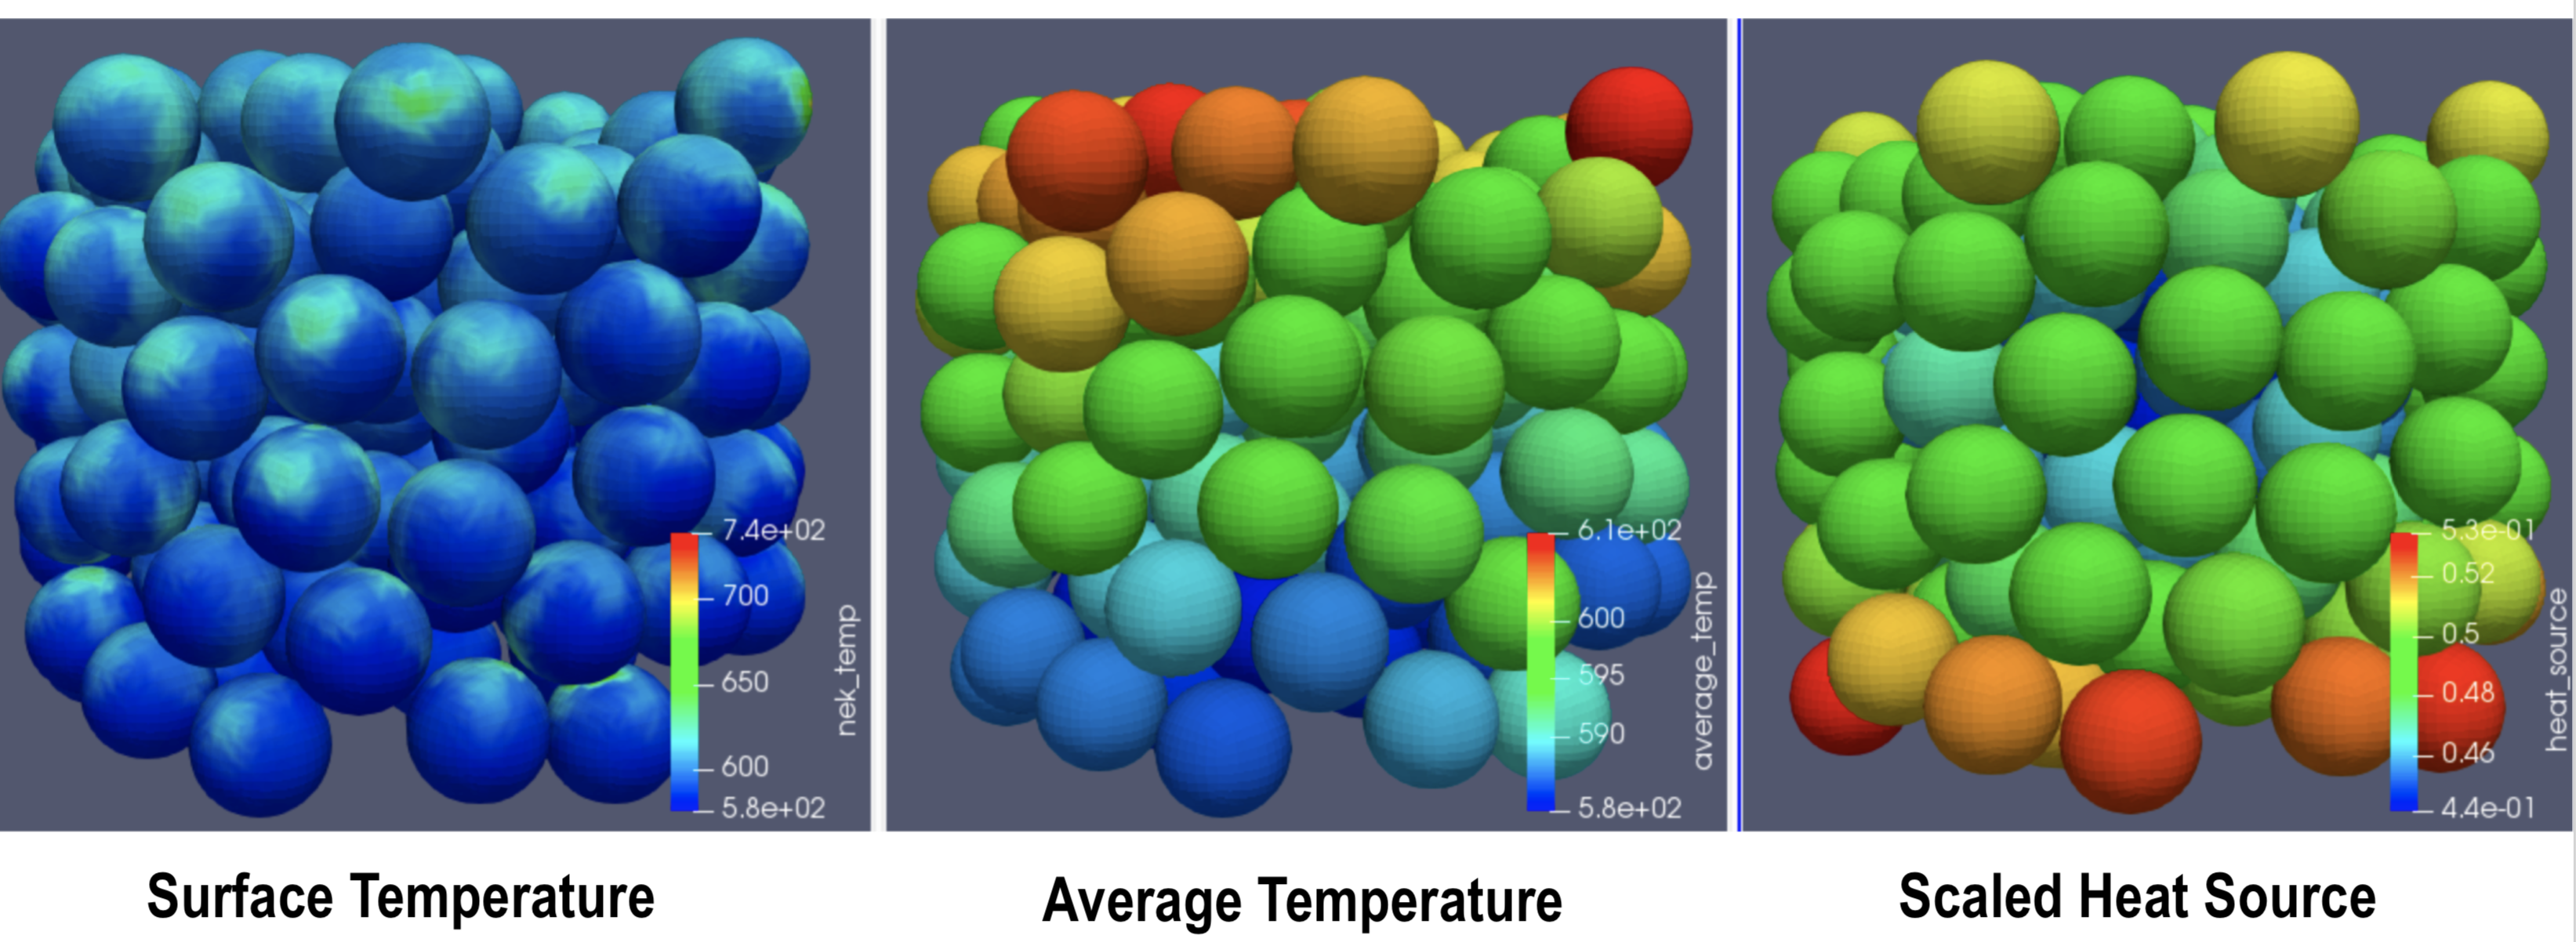
\includegraphics[clip=true,width=0.9\textwidth]{Figures/demo_r1}
\caption{TAMU demo Results. From left to right: snapshots of temperature on surface, average temperature in solid and average heating}
\label{f:dtamu1}
\end{figure}

\begin{figure}[!h]
\centering
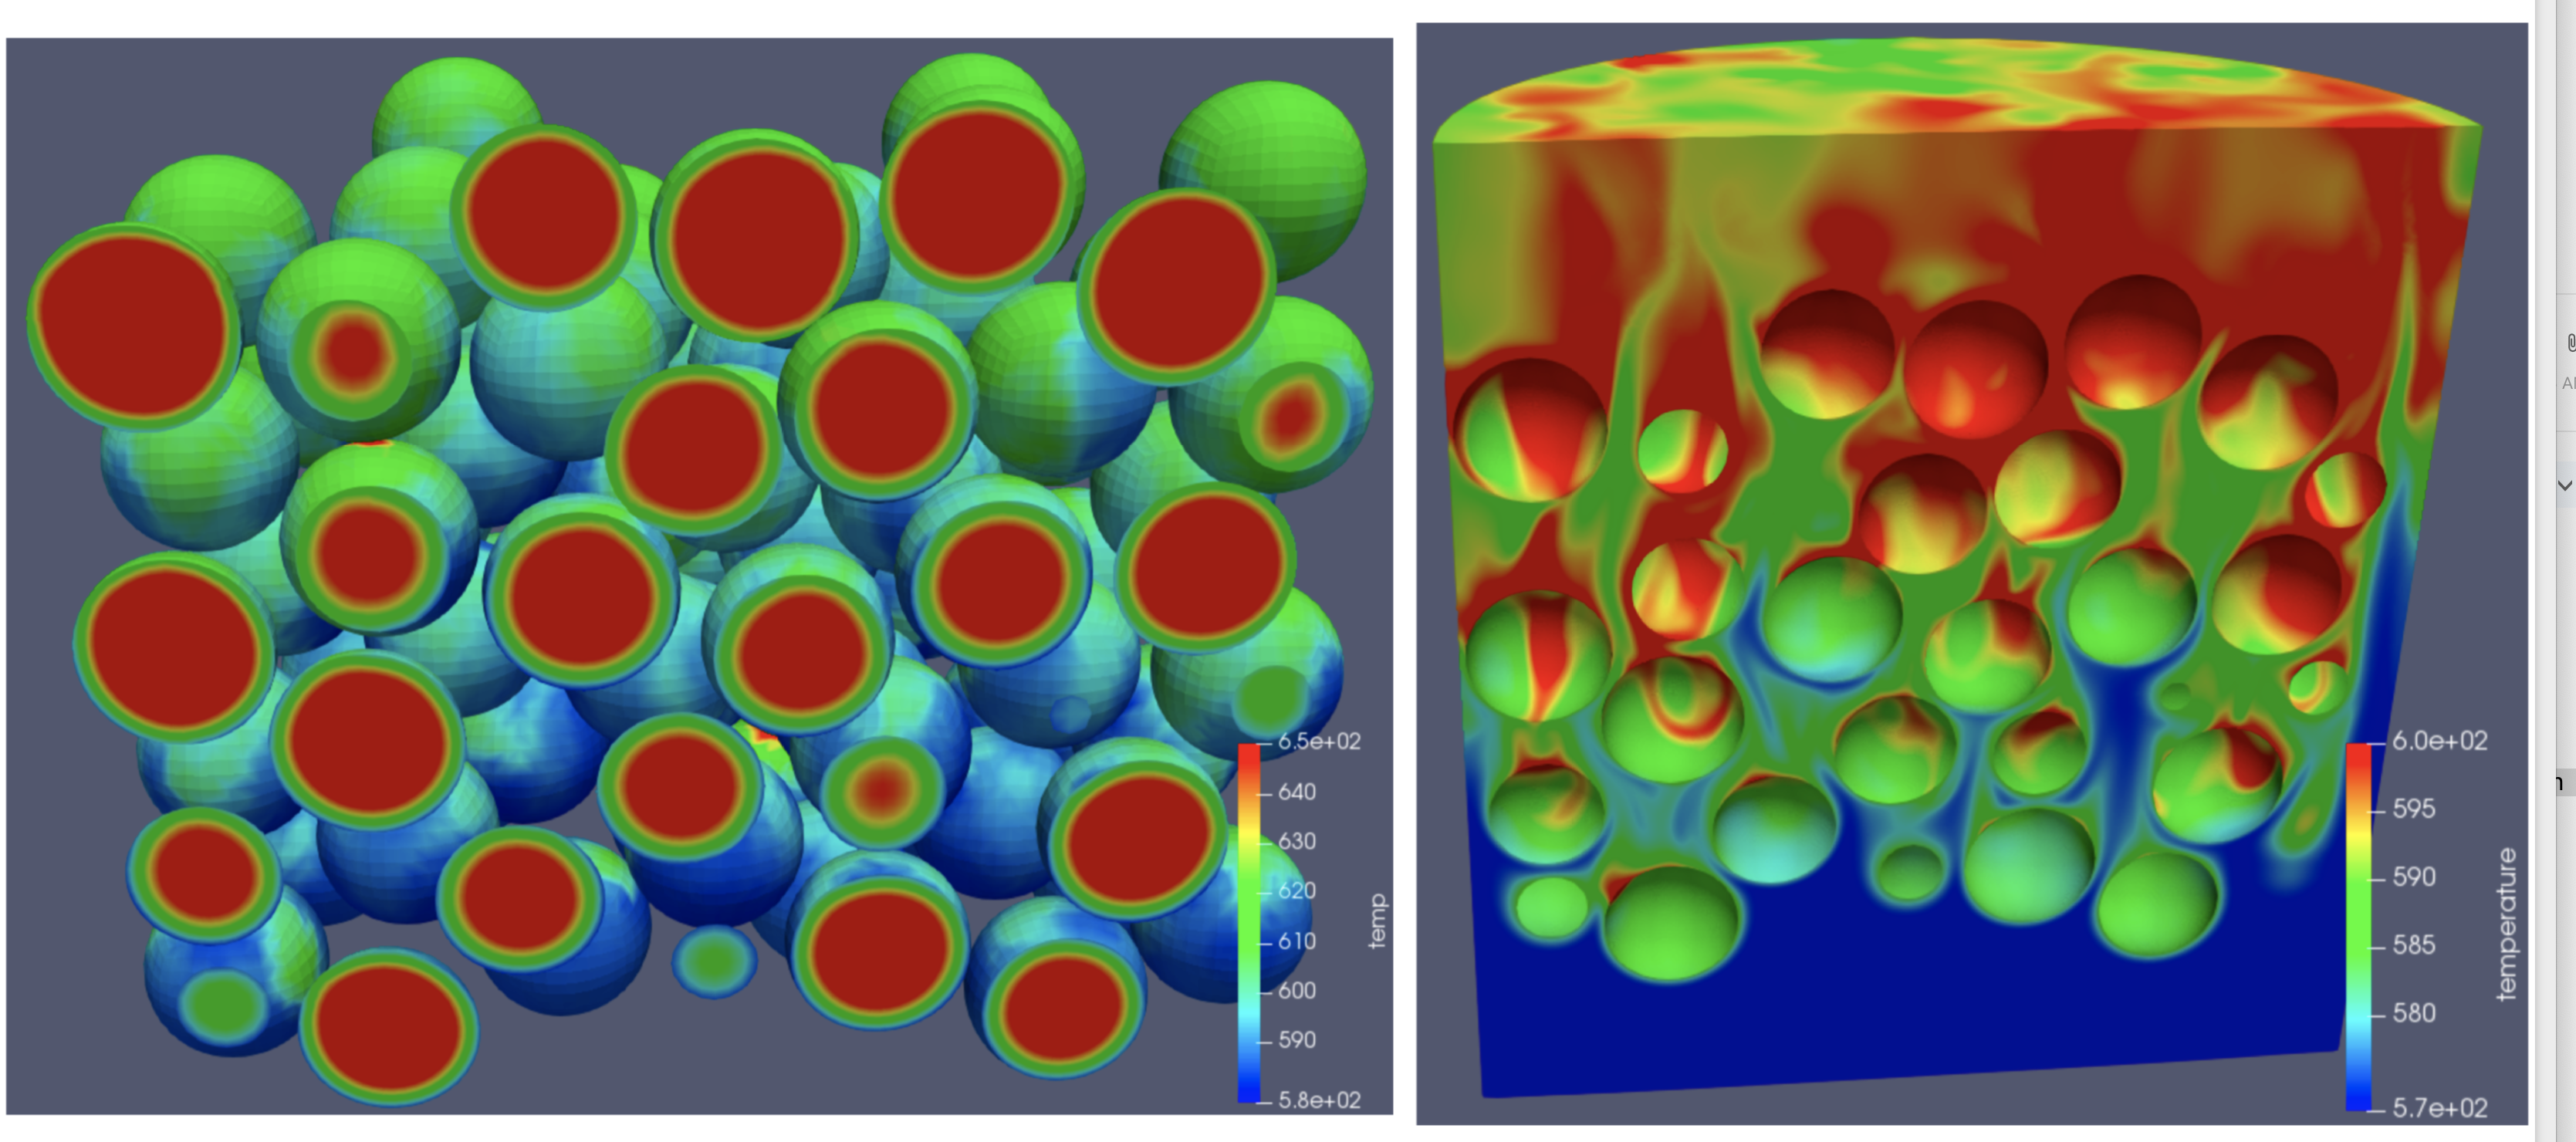
\includegraphics[clip=true,width=0.9\textwidth]{Figures/demo_r2}
\caption{TAMU Demo Results. Right - temperature in the solid. Left - temperature details in the fluid.}
\label{f:dtamu2}
\end{figure}

\subsection{1568 pebbles}

\subsubsection{Numerical Setup}

We also present a case comprising 1568 pebbles. The pebble configuration has
been obtained using a discrete element method (DEM) code~\cite{projectChronoWebSite}.
A major overhaul on the mesh generation for the fluid domain was necessary
to automate as much as possible the process and to reduce the number of elements
per pebble. The new meshing tool is based on a Voronoi cell strategy.
It has allowed us to produce high quality hexahedral meshes while reducing the mesh
count to roughly 300--400 elements per pebble.

An example is provided in Figure~\ref{f:ndemo1} for the 1568
pebble configuration. Higher pebble counts have a similar mesh density.
We note that 1568 pebbles is a significant size for a coupled calculation and
representative of the SANA experiments, for instance.

The principal objective of the new meshing strategy is to reduce the
overall element count so that higher polynomial orders (e.g., $N=7$
to 9) may be effectively employed.   The base elements for the
spectral element method are curvilinear hexahedral (hex) elements
with an effective resolution of $N^3$ points for each of $E$ elements.
A minimum value of $n \approx EN^3$ is required to capture the turbulent
thermal transport.  With a lower element count, $E$, it is possible to
elevate the local approximation order.  $N=7$ is a nearly optimal value
for Nek5000/NekRS because it realizes high throughput with reasonable
element counts and reasonable timestep sizes~\cite{fischer20a}.

The foundation for the new all-hex meshing strategy is to construct
the Voronoi tesselation of the thermal-fluid domain in the void space
between the spheres and vessel walls.  The Voronoi tesselation has
several important properties:
\begin{itemize}
  \item Each Voronoi cell is convex and closed, with cell walls formed
        by facets that bisect the line connecting adjacent sphere centers.
  \item Each facet is a planar convex polygon.
  \item For $\cal N$ spheres, Voronoi tesselation has an expected
        complexity of $O(\cal N)$.
\end{itemize}
Each convex polygon can be tesselated into a set of quadrilaterals
if we permit insertion of a vertex along edges.  For example, if the
facet is a triangle, we insert a vertex on each of the three
edges and then subdivide the triangle into three quads.  Each of these
quads can be projected onto the sphere surface to produce a hex element
that connects the surface to the Voronoi-cell facet.  For a given
sphere, one can refine in the radial direction without having the
refinement propagate through the domain.  The same procedure
can be performed for each Voronoi cell (i.e., sphere), so the
overall complexity is ($O(\cal N)$).

Despite the provably good properties of this approach, a significant concern is
that the Voronoi tesselation my still contain very thin facets (i.e., {\em
slivers}) that lead to poorly conditioned elements.  To overcome this and to
generate a more uniform mesh that has a bounded ratio of longest to shortest
edge we first perform edge collapse on the Voronoi cells.  Any edge that is
shorter than a given tolerance is collaped and its two vertices are fused into
one.  If, after edge collapse, the number of edges on a facet is $<$ 3, the
facet is deleted.   Subsequent to edge collapse, we use {\em vertex insertion}
to ensure that the {\em longest} edge is below a certain threshold.
The risk of edge collapse is that facets lose their planarity and, worse,
might not actually face the sphere that they are nominally bounding.
These situations require some care to recover to ensure that the
resulting all-hex mesh has valid positive Jacobians for each element.

Once the mesh is constructed, it is smoothed using a combination of Laplacian
smoothing and element-Jacobian optimization where the objective function
includes a substantial penalty for negative Jacobians.

\begin{figure}[!h]
\centering
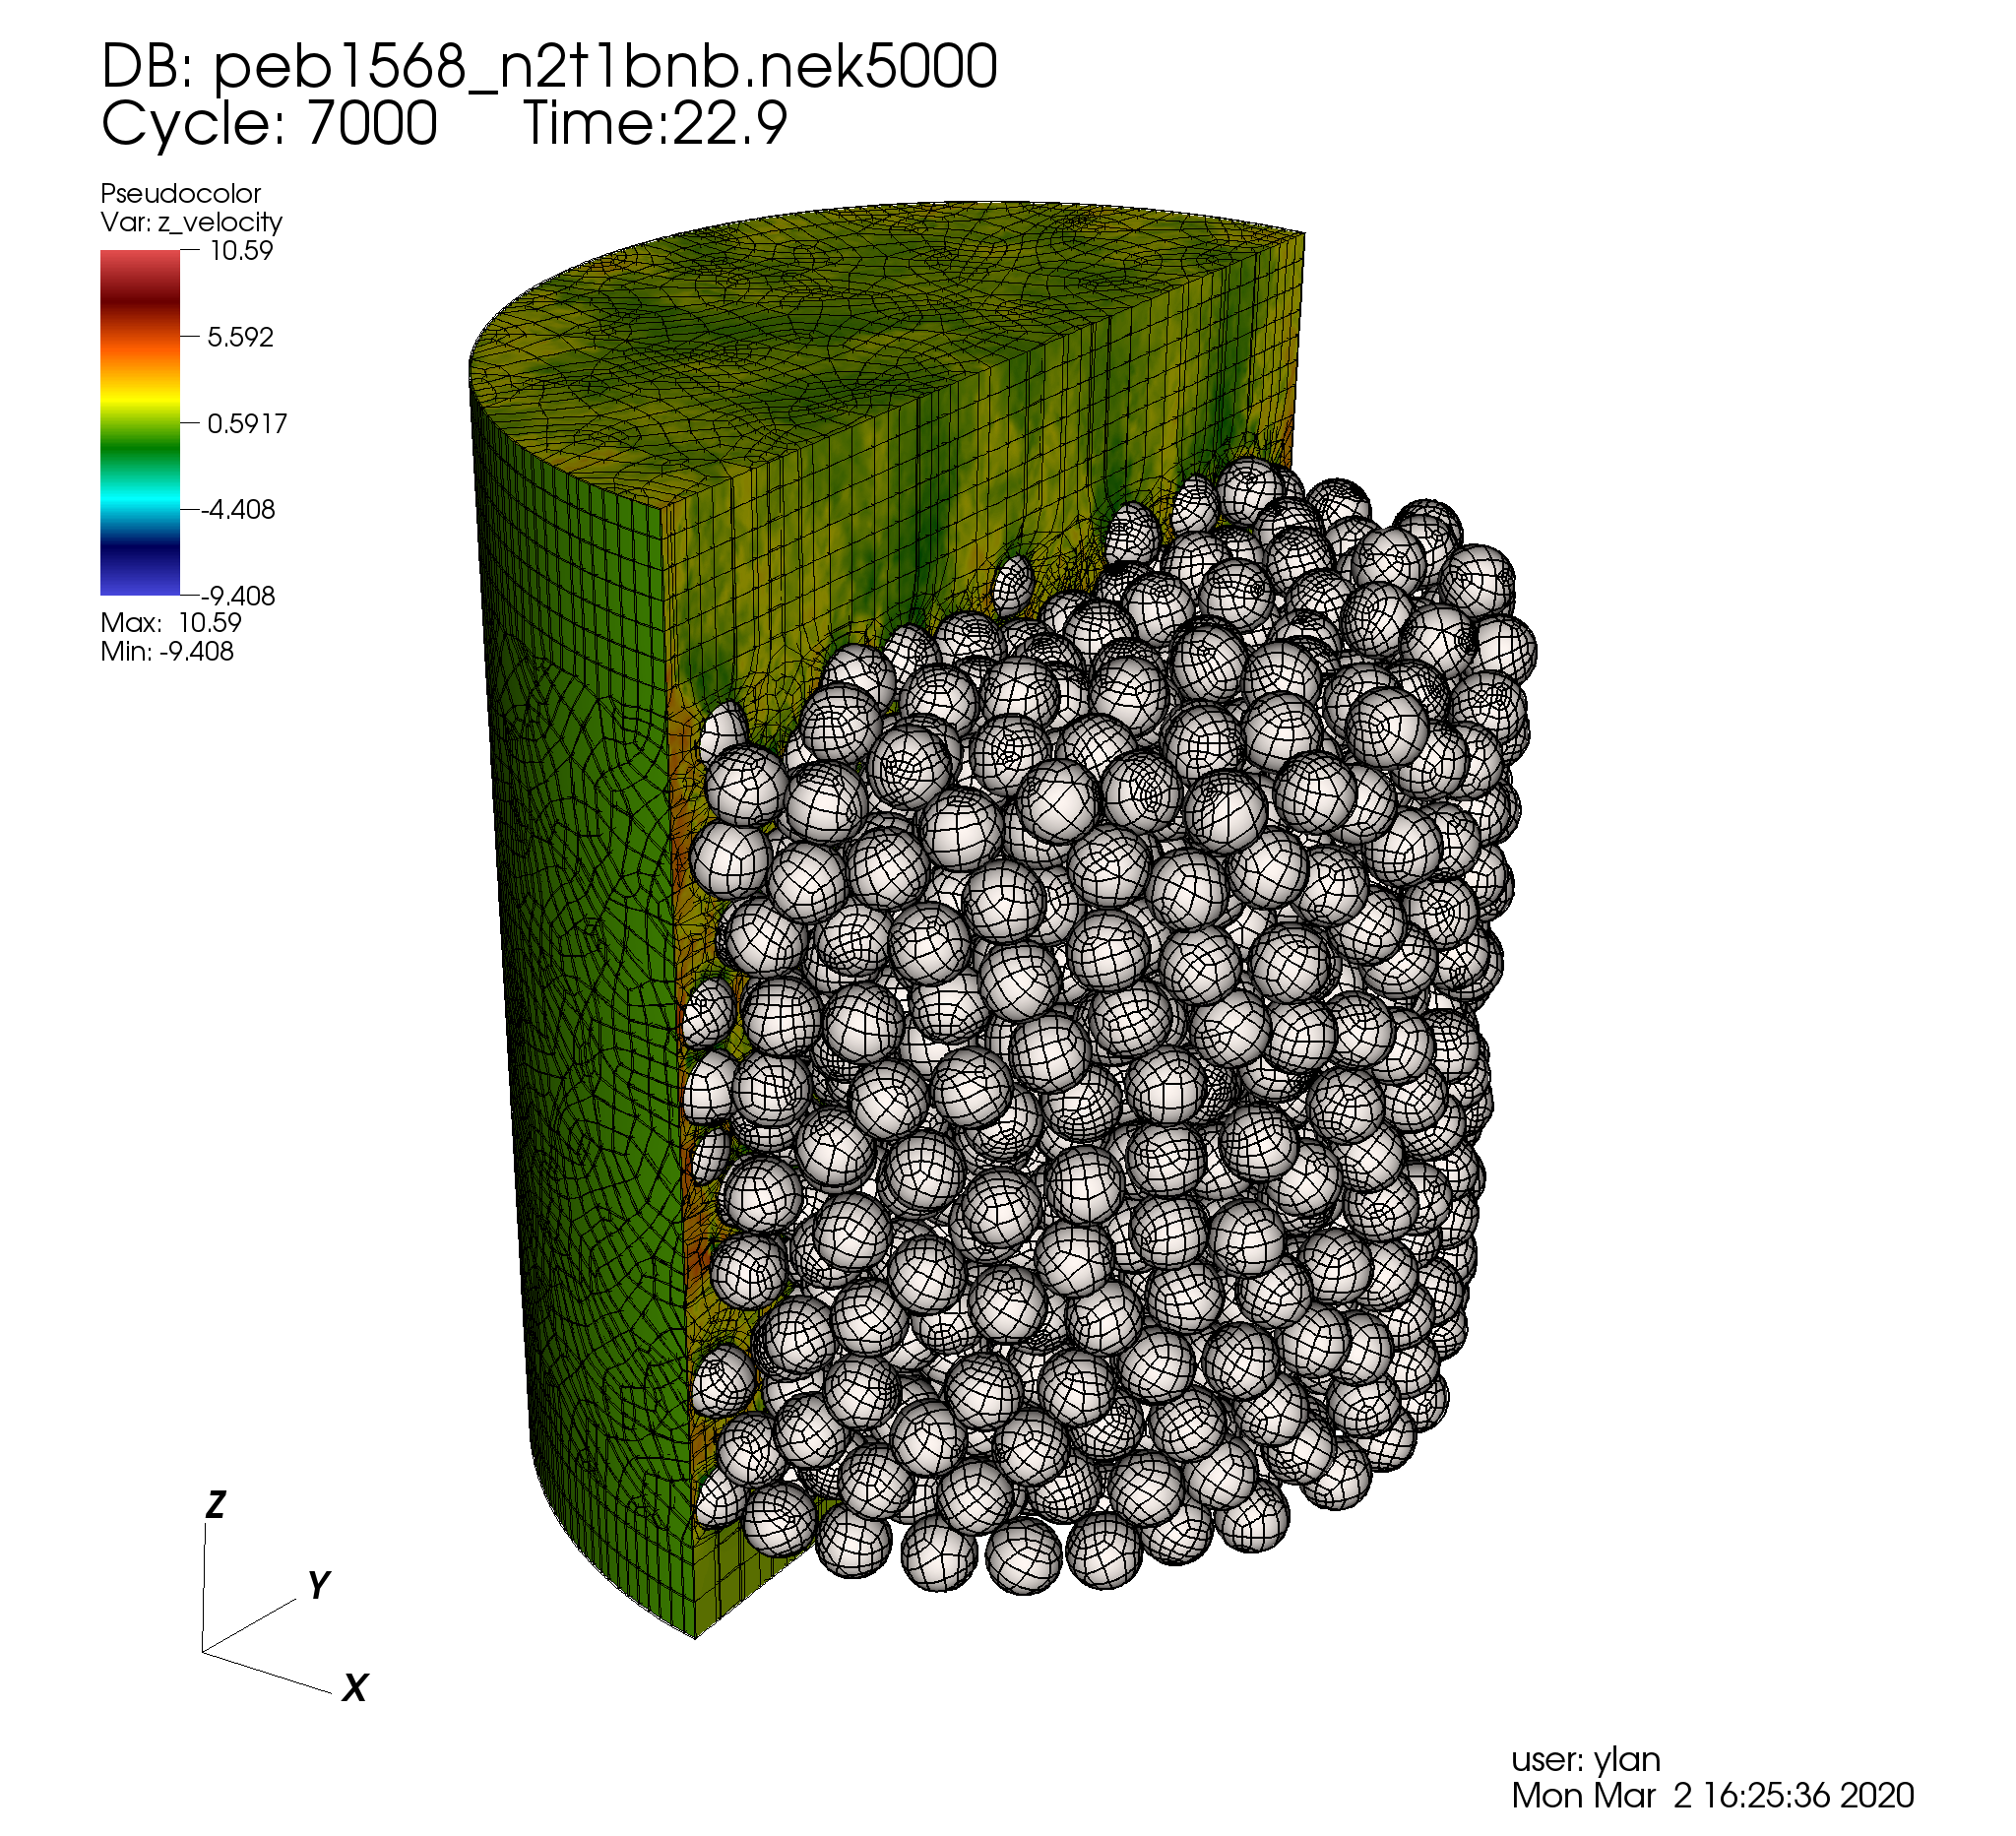
\includegraphics[clip=true,width=0.9\textwidth]{Figures/ndemo_r1}
\caption{NekRS mesh for 1568 pebble configuration using 524,386 spectral elements. }
\label{f:ndemo1}
\end{figure}

For this demonstrations, the sizes and composition of the TRISO particles were based on TRISO manufactured at INL, following the practice established in the validation section. Though these particles were developed for the Advanced Gas Reactor (AGR) fuel, particles with the same specifications are used for FHR test reactors and computation benchmarks. The sizes and compositions of the pebbles were taken from the Mark-1 FHR reactor constructed at UC Berkeley. For BISON and the demonstration problem under consideration, we consider only the conduction equation and as such it is a relatively straightforward setup. Properties are constant and adapted from available correlations. The mesh for a single sphere is generated and replicated at run time. The same mesh is used for the mesh tallies in OpenMC.

\subsubsection{Results}

The model described in the previous section has been run on 12 and 20 nodes of Summit, with 6 MPI ranks on each node, corresponding to the 6 GPUs on each node. The OpenMC and BISON models are designed to run on CPU while the NekRS model runs on the GPU. Stand-alone NekRS simulations have been run first up to 25 convective time units to develop turbulence, the results of which are shown in Figure~\ref{f:ndemo3} using a Large Eddy Simulation (LES) approach.

A restart file has then been generated and used to restart a transient simulation in Cardinal representing heat-up of the pebbles. The time step has been fixed to $5\times 10^{-4}$ s in both BISON and NekRS. The temperature at time zero has been set to 300 $^{\circ}$C everywhere. Figure~\ref{f:ndemo4} presents the temperature at the surface of the pebbles in BISON at three points in time. The simulations took 2.5 s per coupled time step on 20 nodes, requiring transfer between physics at each time step. However this could be greatly optimized by relaxing the requirement, as data transfer from GPU to CPU should be minimized as much as possible.

\begin{figure}[!h]
\centering
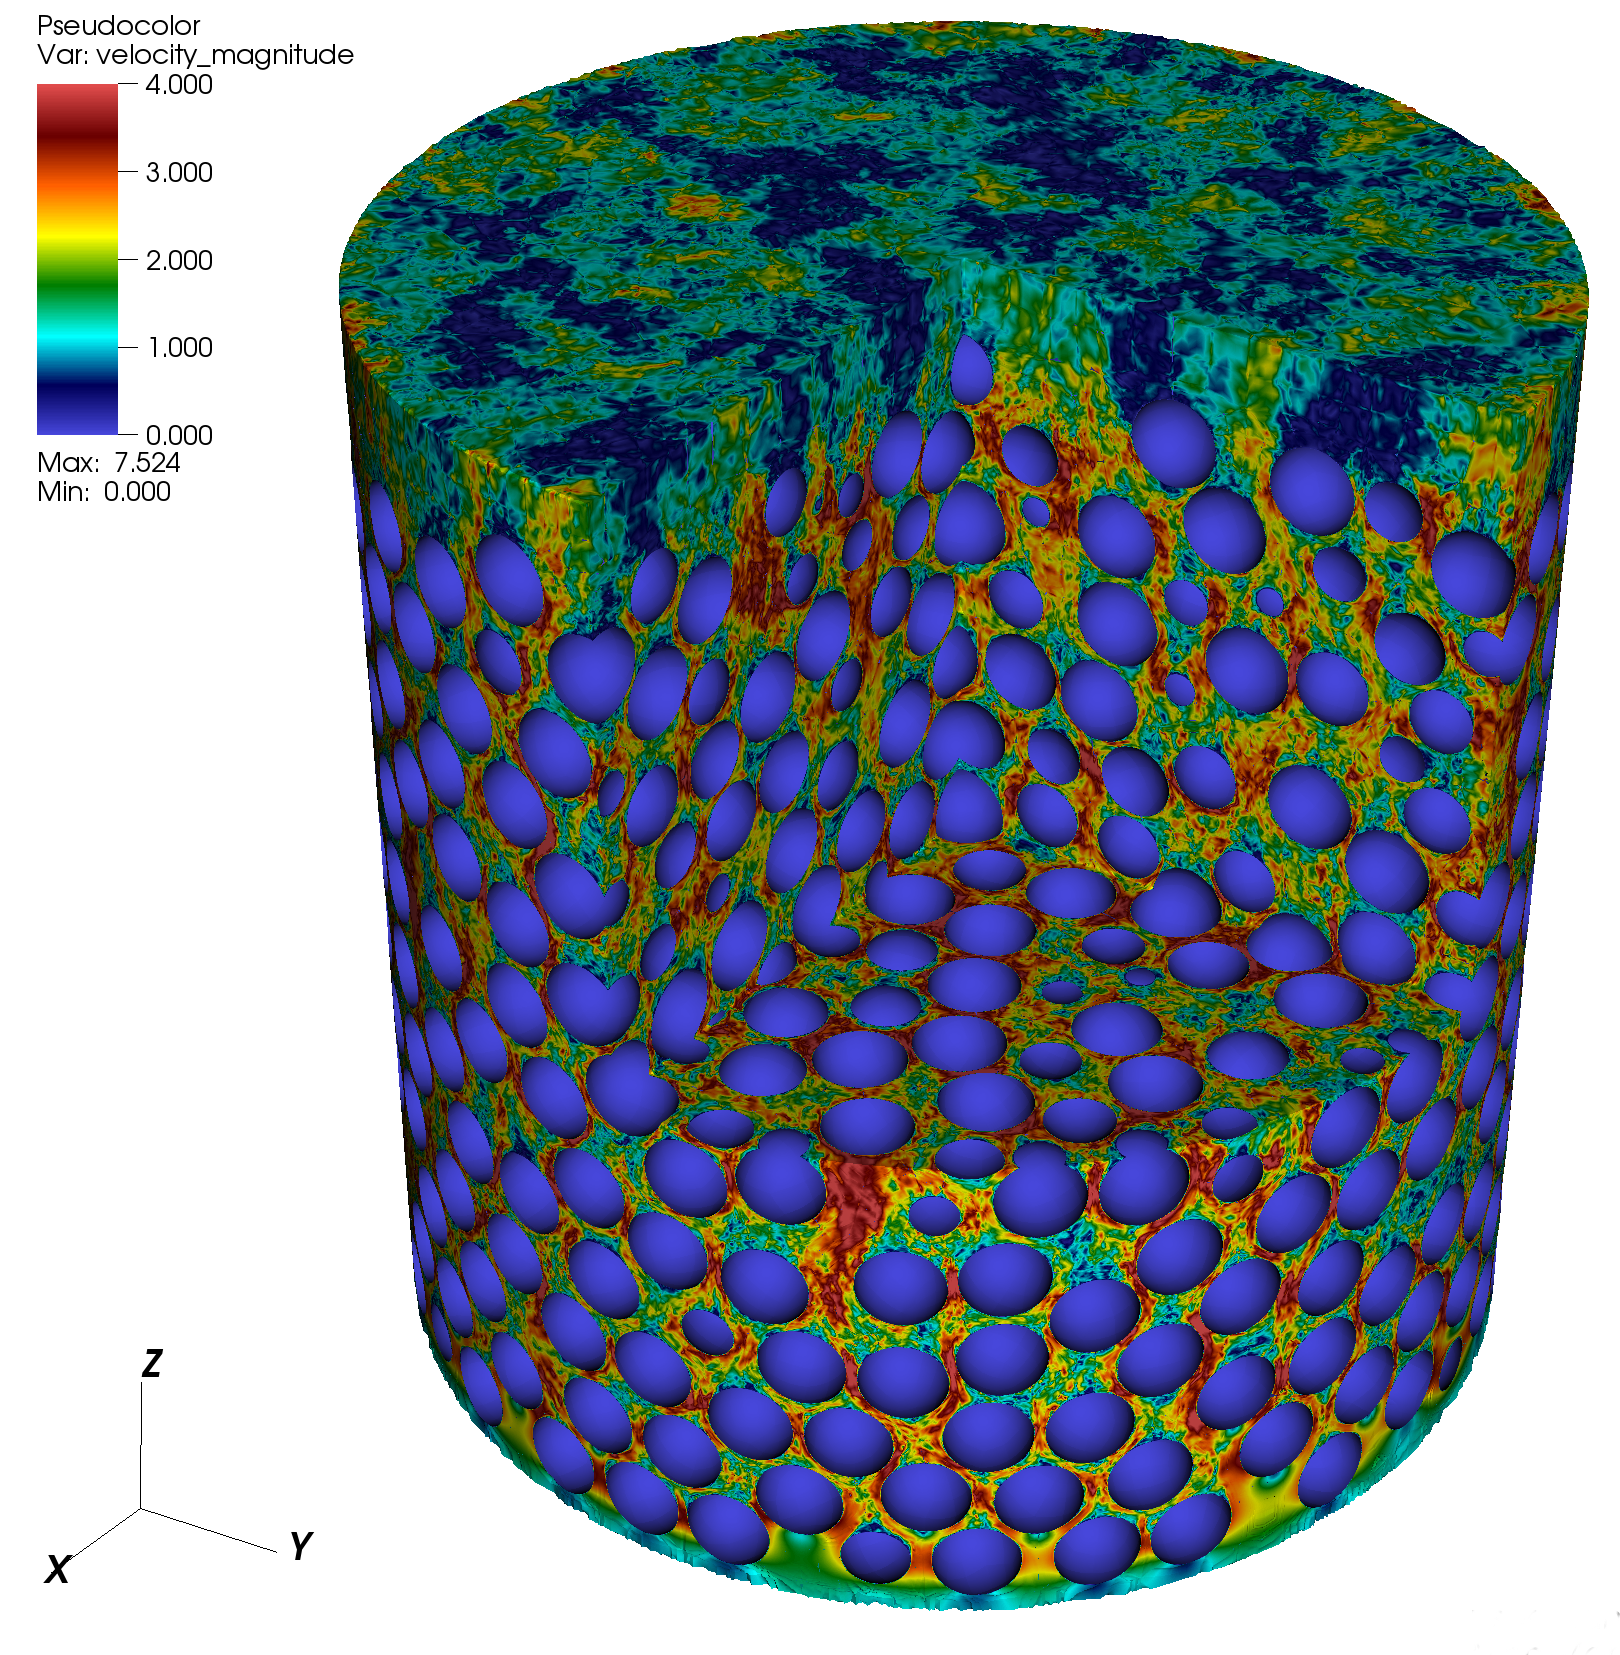
\includegraphics[clip=true,width=0.9\textwidth]{Figures/ndemo_r3}
\caption{NekRS results for the velocity field.}
\label{f:ndemo3}
\end{figure}


\begin{figure}[!h]
\centering
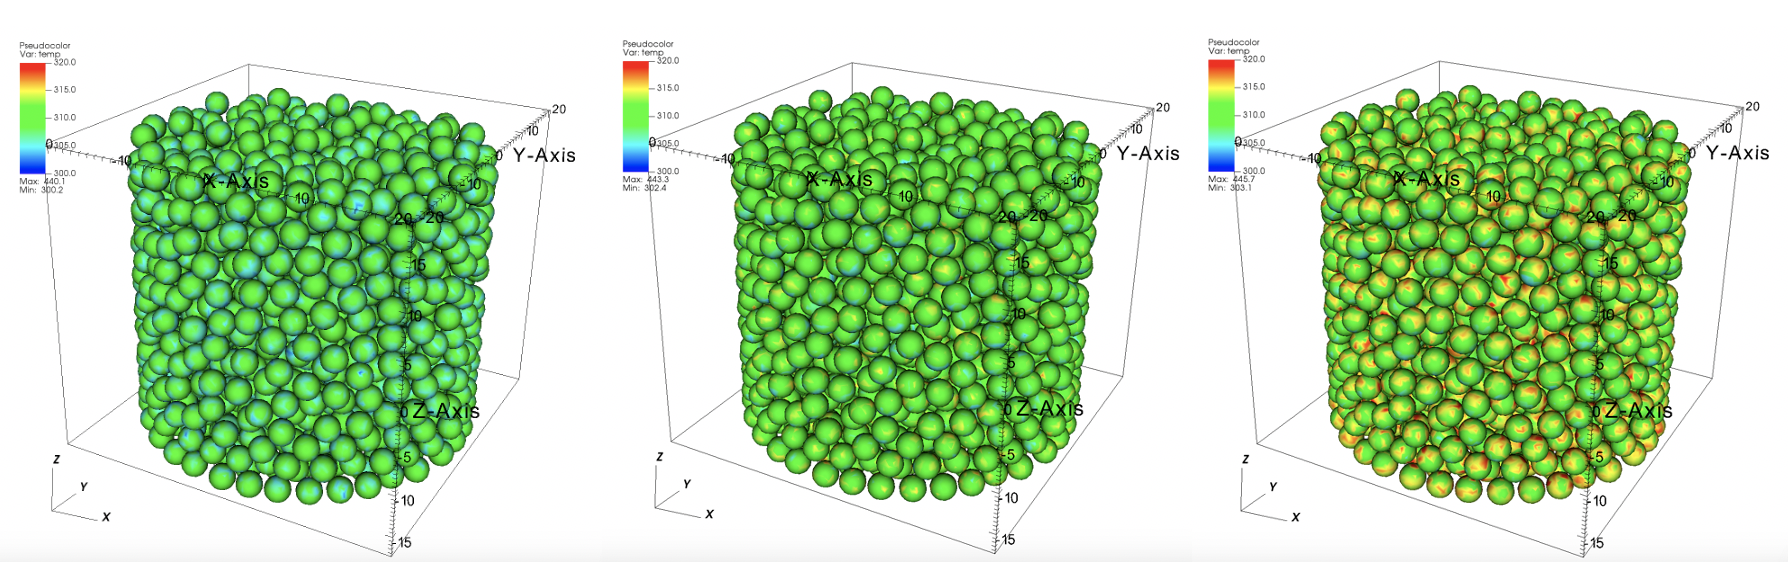
\includegraphics[clip=true,width=0.9\textwidth]{Figures/ndemo_r4}
\caption{Temperature result for the pebble surface temperature at three points in time.}
\label{f:ndemo4}
\end{figure}

The results of OpenMC simulations coupled with the heat conduction module are
shown in Figures~\ref{f:1568_openmc_heat_source} and
~\ref{f:1568_openmc_temperatures} with the same time step parameters as the
NekRS simulations described above. An eigenvalue simulation using 150 batches
with 50 inactive batches was executed in each time step. 50,000 particles per
batch were used to converge the pebble-averaged heat source from the OpenMC cell
tally while the unstructured mesh heat source tally required 500,000 particles
per batch to produce the heat source presented here. Production simulations may
require an even higher number of particles per batch to more tightly converge
the heating distribution when using the unstructured mesh heat source due to the
decreased number of samples per source particle in the tally bins.
Figure~\ref{f:1568_openmc_temperatures_single_pebble} demonstrates the effect of
the improved spatial resolution provided by the unstructured mesh heat source
from OpenMC on the temperature distribution within a representative pebble. In
the case of the pebble-averaged heat source the temperature profile is
symmetric, reflecting the uniform heat source applied in that region, while an
asymmetry can be seen in the profile generated from the unstructured mesh heat
source indicating that the improved spatial resolution of the source has an
impact on the temperature distribution in the solid and will in turn affect the
resulting heat transfer to the fluid.

\begin{figure}[!h]
\centering
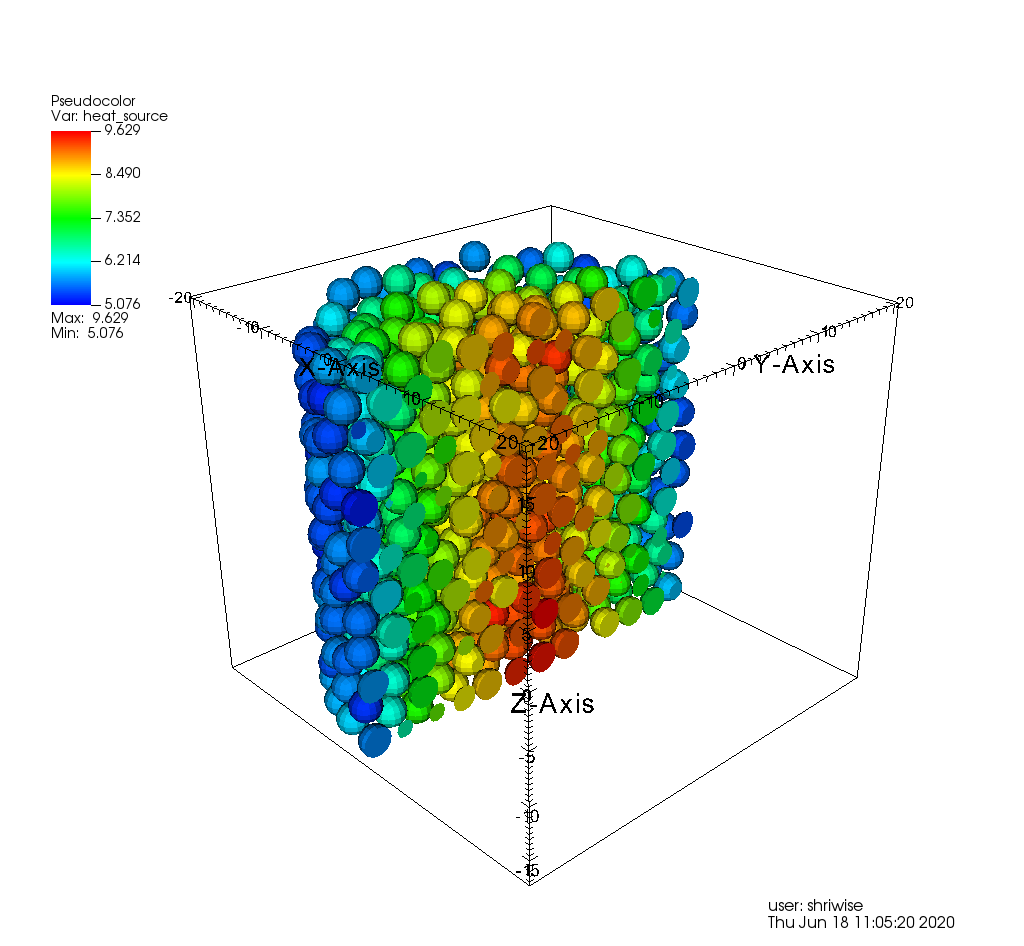
\includegraphics[clip=true,width=0.48\textwidth]{Figures/openmc_cell_heat_source}
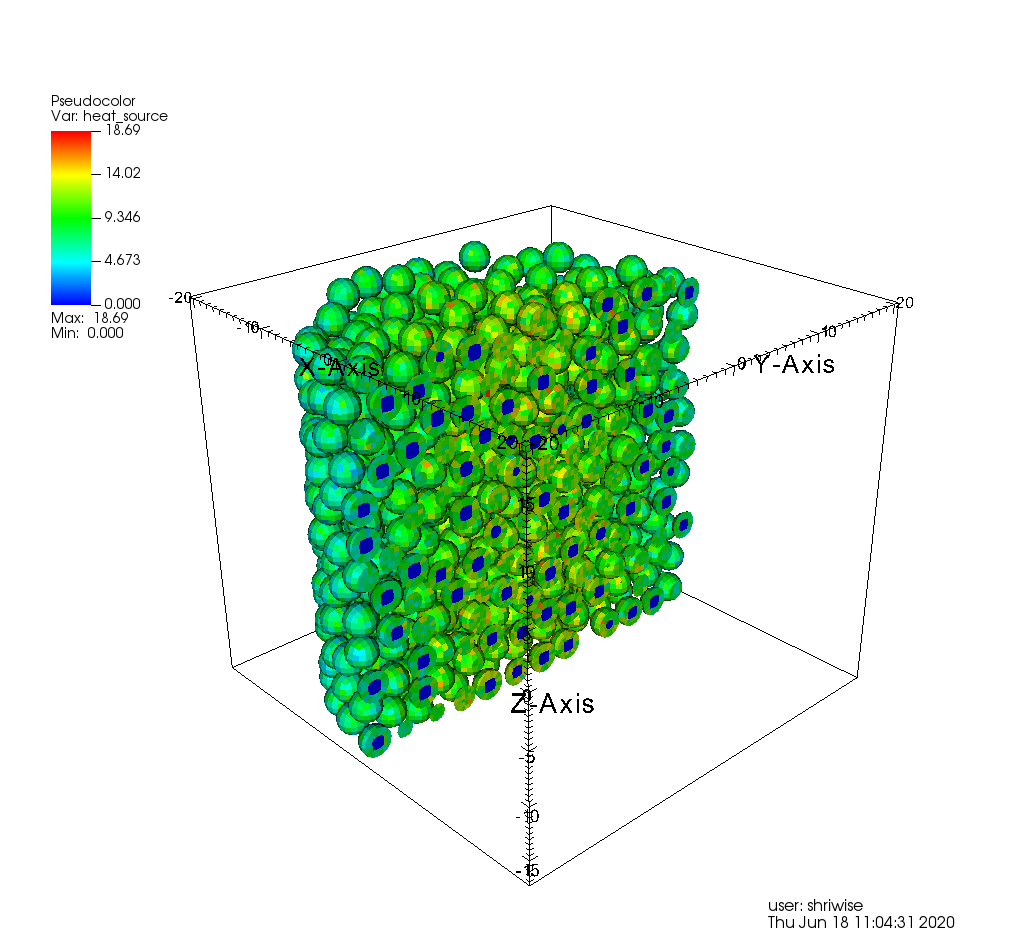
\includegraphics[clip=true,width=0.48\textwidth]{Figures/openmc_mesh_heat_source}
\caption{Left: Heat source using the original cell tallies to produces an average heat source per-pebble. Right: Heat source produced using an OpenMC unstructured mesh tally.}
\label{f:1568_openmc_heat_source}
\end{figure}

\begin{figure}[!h]
\centering
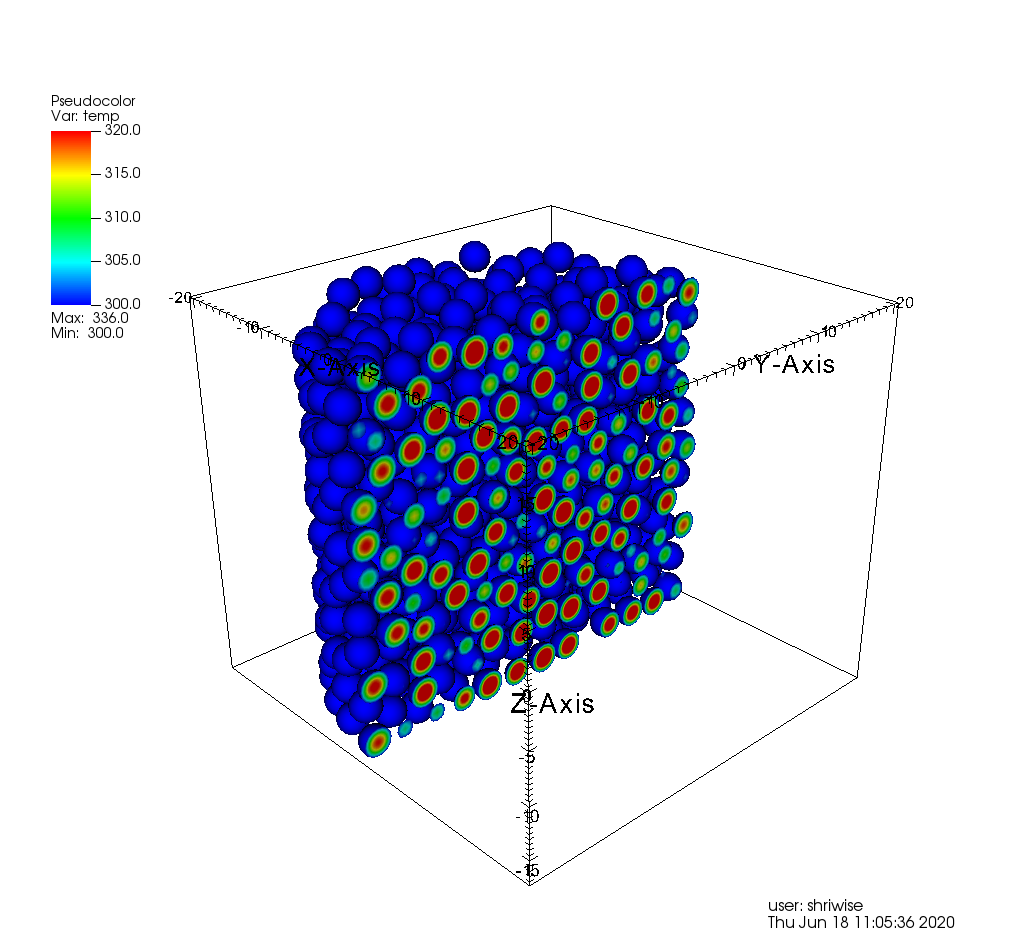
\includegraphics[clip=true,width=0.48\textwidth]{Figures/openmc_cell_temperature}
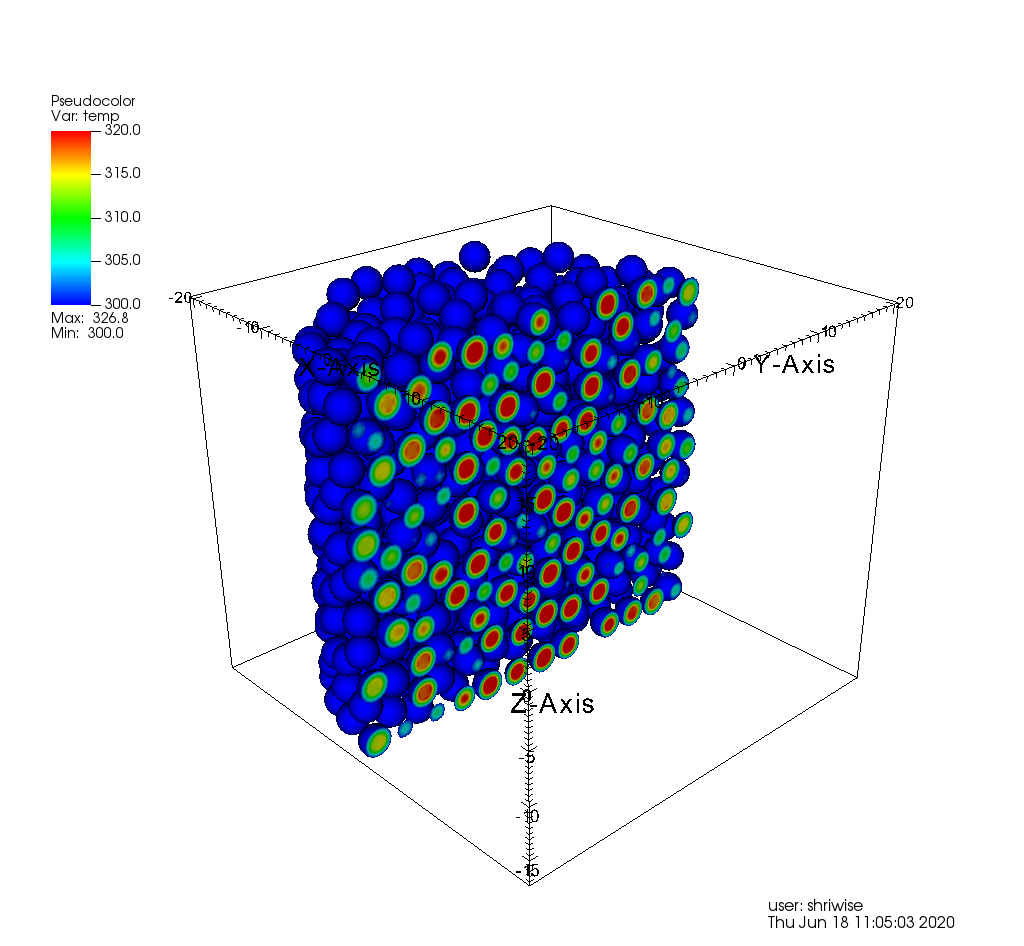
\includegraphics[clip=true,width=0.48\textwidth]{Figures/openmc_mesh_temperature}
\caption{Left: Temperature in the solid resulting from the cell-based heating tally. Right: Temperature in the solid resulting from the unstructured mesh heating tally in OpenMC.}
\label{f:1568_openmc_temperatures}
\end{figure}

\begin{figure}[!h]
\centering
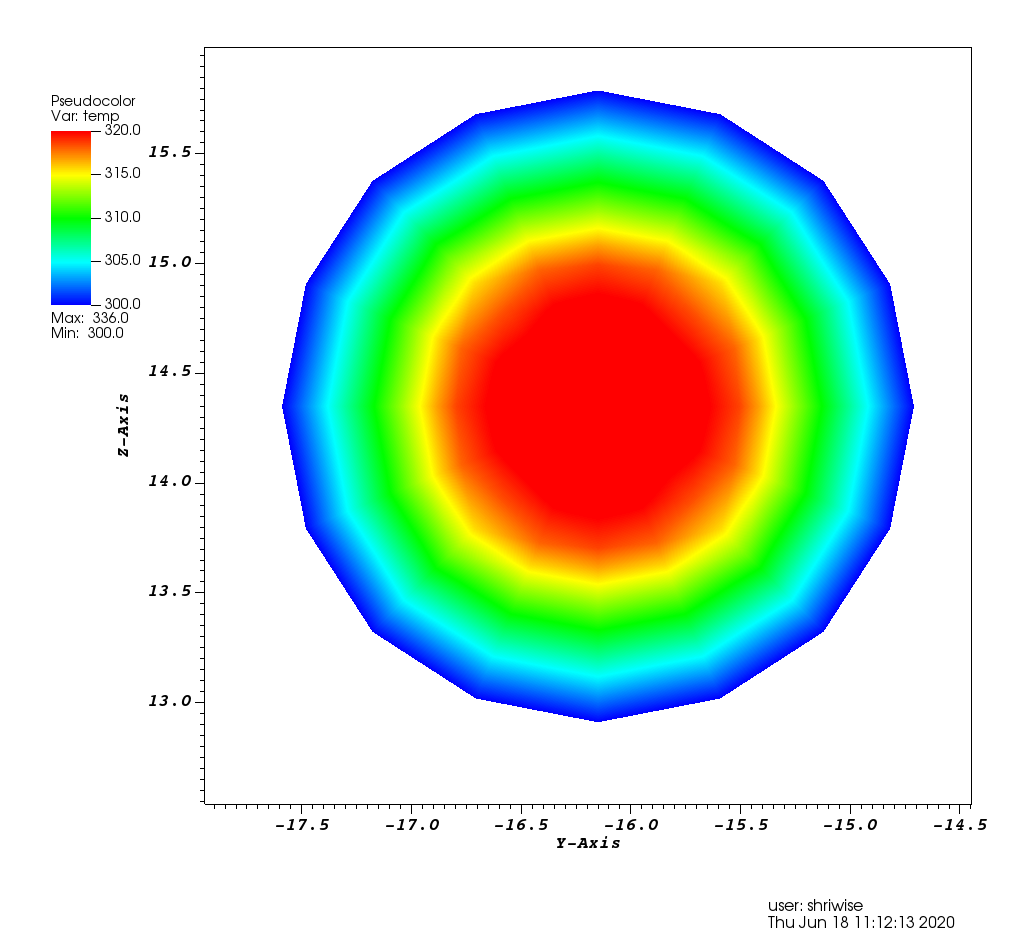
\includegraphics[clip=true,width=0.48\textwidth]{Figures/openmc_cell_temperature_zoomed}
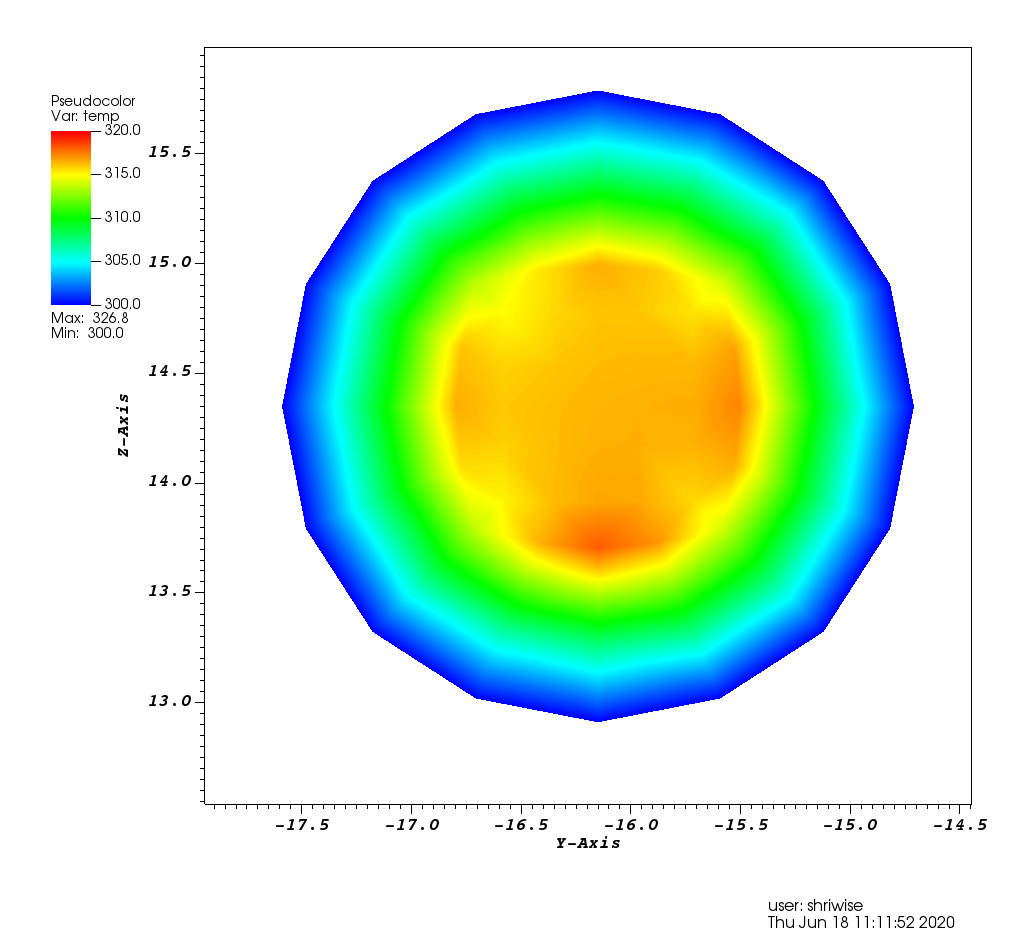
\includegraphics[clip=true,width=0.48\textwidth]{Figures/openmc_mesh_temperature_zoomed}
\caption{Temperature profiles of the same pebble in the 1568 pebble demo using the pebble-averaged heating (left) and the unstructured mesh heating (right).}
\label{f:1568_openmc_temperatures_single_pebble}
\end{figure}

\subsection{Projection to full core}

20 nodes of Summit represents less than 1\% of the computing power available on Summit. We estimate that 80\% of the machine will be sufficient to perform full core calculation in FHRs corresponding to 300,000 pebbles.
